\documentclass{article}
\usepackage{tikz}
\usetikzlibrary{decorations.markings}
\newif\iflabrev
\begin{document}
%P1
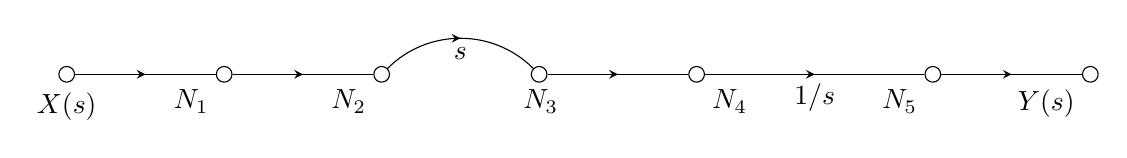
\begin{tikzpicture}
[
label revd/.is if=labrev,
amark/.style={
            decoration={             
                        markings,   
                        mark=at position {0.5} with { 
                                    \arrow{stealth},
                                    \iflabrev \node[above] {#1};\else \node[below] {#1};\fi
                        }
            },
            postaction={decorate}
},
terminal/.style 2 args={draw,circle,inner sep=2pt,label={#1:#2}},
]

%Place the nodes
\node[terminal={below}{$X(s)$}] (a) at (0,0) {};
\node[terminal={below left}{$N_1$}] (b) at (2cm,0) {};
\node[terminal={below left}{$N_2$}] (c) at (4cm,0) {};
\node[terminal={[xshift=-4mm]below right}{$N_3$}] (d) at (6cm,0) {};
\node[terminal={below right}{$N_4$}] (e) at (8cm,0) {};
\node[terminal={below left}{$N_5$}] (f) at (11cm,0) {};
\node[terminal={below left}{$Y(s)$}] (g) at (13cm,0) {};
%Draw the connections
\draw[amark=$ $] (a) to (b);
\draw[amark=$ $] (b) to (c);
\draw[amark=$s$] (c) to[bend left=45] (d);
\draw[amark=$1/s$] (e) to (f);
\draw[amark=$ $] (f) to (g);
\draw[amark=$ $] (d) to (e);
\end{tikzpicture}
\end{document}